\documentclass[11pt]{article}

    \usepackage[breakable]{tcolorbox}
    \usepackage{parskip} % Stop auto-indenting (to mimic markdown behaviour)
    

    % Basic figure setup, for now with no caption control since it's done
    % automatically by Pandoc (which extracts ![](path) syntax from Markdown).
    \usepackage{graphicx}
    % Maintain compatibility with old templates. Remove in nbconvert 6.0
    \let\Oldincludegraphics\includegraphics
    % Ensure that by default, figures have no caption (until we provide a
    % proper Figure object with a Caption API and a way to capture that
    % in the conversion process - todo).
    \usepackage{caption}
    \DeclareCaptionFormat{nocaption}{}
    \captionsetup{format=nocaption,aboveskip=0pt,belowskip=0pt}

    \usepackage{float}
    \floatplacement{figure}{H} % forces figures to be placed at the correct location
    \usepackage{xcolor} % Allow colors to be defined
    \usepackage{enumerate} % Needed for markdown enumerations to work
    \usepackage{geometry} % Used to adjust the document margins
    \usepackage{amsmath} % Equations
    \usepackage{amssymb} % Equations
    \usepackage{physics} % Equations
    \usepackage{textcomp} % defines textquotesingle
    % Hack from http://tex.stackexchange.com/a/47451/13684:
    \AtBeginDocument{%
        \def\PYZsq{\textquotesingle}% Upright quotes in Pygmentized code
    }
    \usepackage{upquote} % Upright quotes for verbatim code
    \usepackage{eurosym} % defines \euro

    \usepackage{iftex}
    \ifPDFTeX
        \usepackage[T1]{fontenc}
        \IfFileExists{alphabeta.sty}{
              \usepackage{alphabeta}
          }{
              \usepackage[mathletters]{ucs}
              \usepackage[utf8x]{inputenc}
          }
    \else
        \usepackage{fontspec}
        \usepackage{unicode-math}
    \fi

    \usepackage{fancyvrb} % verbatim replacement that allows latex
    \usepackage{grffile} % extends the file name processing of package graphics
                         % to support a larger range
    \makeatletter % fix for old versions of grffile with XeLaTeX
    \@ifpackagelater{grffile}{2019/11/01}
    {
      % Do nothing on new versions
    }
    {
      \def\Gread@@xetex#1{%
        \IfFileExists{"\Gin@base".bb}%
        {\Gread@eps{\Gin@base.bb}}%
        {\Gread@@xetex@aux#1}%
      }
    }
    \makeatother
    \usepackage[Export]{adjustbox} % Used to constrain images to a maximum size
    \adjustboxset{max size={0.9\linewidth}{0.9\paperheight}}

    % The hyperref package gives us a pdf with properly built
    % internal navigation ('pdf bookmarks' for the table of contents,
    % internal cross-reference links, web links for URLs, etc.)
    \usepackage{hyperref}
    % The default LaTeX title has an obnoxious amount of whitespace. By default,
    % titling removes some of it. It also provides customization options.
    \usepackage{titling}
    \usepackage{longtable} % longtable support required by pandoc >1.10
    \usepackage{booktabs}  % table support for pandoc > 1.12.2
    \usepackage{array}     % table support for pandoc >= 2.11.3
    \usepackage{calc}      % table minipage width calculation for pandoc >= 2.11.1
    \usepackage[inline]{enumitem} % IRkernel/repr support (it uses the enumerate* environment)
    \usepackage[normalem]{ulem} % ulem is needed to support strikethroughs (\sout)
                                % normalem makes italics be italics, not underlines
    \usepackage{mathrsfs}
    

    
    % Colors for the hyperref package
    \definecolor{urlcolor}{rgb}{0,.145,.698}
    \definecolor{linkcolor}{rgb}{.71,0.21,0.01}
    \definecolor{citecolor}{rgb}{.12,.54,.11}

    % ANSI colors
    \definecolor{ansi-black}{HTML}{3E424D}
    \definecolor{ansi-black-intense}{HTML}{282C36}
    \definecolor{ansi-red}{HTML}{E75C58}
    \definecolor{ansi-red-intense}{HTML}{B22B31}
    \definecolor{ansi-green}{HTML}{00A250}
    \definecolor{ansi-green-intense}{HTML}{007427}
    \definecolor{ansi-yellow}{HTML}{DDB62B}
    \definecolor{ansi-yellow-intense}{HTML}{B27D12}
    \definecolor{ansi-blue}{HTML}{208FFB}
    \definecolor{ansi-blue-intense}{HTML}{0065CA}
    \definecolor{ansi-magenta}{HTML}{D160C4}
    \definecolor{ansi-magenta-intense}{HTML}{A03196}
    \definecolor{ansi-cyan}{HTML}{60C6C8}
    \definecolor{ansi-cyan-intense}{HTML}{258F8F}
    \definecolor{ansi-white}{HTML}{C5C1B4}
    \definecolor{ansi-white-intense}{HTML}{A1A6B2}
    \definecolor{ansi-default-inverse-fg}{HTML}{FFFFFF}
    \definecolor{ansi-default-inverse-bg}{HTML}{000000}

    % common color for the border for error outputs.
    \definecolor{outerrorbackground}{HTML}{FFDFDF}

    % commands and environments needed by pandoc snippets
    % extracted from the output of `pandoc -s`
    \providecommand{\tightlist}{%
      \setlength{\itemsep}{0pt}\setlength{\parskip}{0pt}}
    \DefineVerbatimEnvironment{Highlighting}{Verbatim}{commandchars=\\\{\}}
    % Add ',fontsize=\small' for more characters per line
    \newenvironment{Shaded}{}{}
    \newcommand{\KeywordTok}[1]{\textcolor[rgb]{0.00,0.44,0.13}{\textbf{{#1}}}}
    \newcommand{\DataTypeTok}[1]{\textcolor[rgb]{0.56,0.13,0.00}{{#1}}}
    \newcommand{\DecValTok}[1]{\textcolor[rgb]{0.25,0.63,0.44}{{#1}}}
    \newcommand{\BaseNTok}[1]{\textcolor[rgb]{0.25,0.63,0.44}{{#1}}}
    \newcommand{\FloatTok}[1]{\textcolor[rgb]{0.25,0.63,0.44}{{#1}}}
    \newcommand{\CharTok}[1]{\textcolor[rgb]{0.25,0.44,0.63}{{#1}}}
    \newcommand{\StringTok}[1]{\textcolor[rgb]{0.25,0.44,0.63}{{#1}}}
    \newcommand{\CommentTok}[1]{\textcolor[rgb]{0.38,0.63,0.69}{\textit{{#1}}}}
    \newcommand{\OtherTok}[1]{\textcolor[rgb]{0.00,0.44,0.13}{{#1}}}
    \newcommand{\AlertTok}[1]{\textcolor[rgb]{1.00,0.00,0.00}{\textbf{{#1}}}}
    \newcommand{\FunctionTok}[1]{\textcolor[rgb]{0.02,0.16,0.49}{{#1}}}
    \newcommand{\RegionMarkerTok}[1]{{#1}}
    \newcommand{\ErrorTok}[1]{\textcolor[rgb]{1.00,0.00,0.00}{\textbf{{#1}}}}
    \newcommand{\NormalTok}[1]{{#1}}

    % Additional commands for more recent versions of Pandoc
    \newcommand{\ConstantTok}[1]{\textcolor[rgb]{0.53,0.00,0.00}{{#1}}}
    \newcommand{\SpecialCharTok}[1]{\textcolor[rgb]{0.25,0.44,0.63}{{#1}}}
    \newcommand{\VerbatimStringTok}[1]{\textcolor[rgb]{0.25,0.44,0.63}{{#1}}}
    \newcommand{\SpecialStringTok}[1]{\textcolor[rgb]{0.73,0.40,0.53}{{#1}}}
    \newcommand{\ImportTok}[1]{{#1}}
    \newcommand{\DocumentationTok}[1]{\textcolor[rgb]{0.73,0.13,0.13}{\textit{{#1}}}}
    \newcommand{\AnnotationTok}[1]{\textcolor[rgb]{0.38,0.63,0.69}{\textbf{\textit{{#1}}}}}
    \newcommand{\CommentVarTok}[1]{\textcolor[rgb]{0.38,0.63,0.69}{\textbf{\textit{{#1}}}}}
    \newcommand{\VariableTok}[1]{\textcolor[rgb]{0.10,0.09,0.49}{{#1}}}
    \newcommand{\ControlFlowTok}[1]{\textcolor[rgb]{0.00,0.44,0.13}{\textbf{{#1}}}}
    \newcommand{\OperatorTok}[1]{\textcolor[rgb]{0.40,0.40,0.40}{{#1}}}
    \newcommand{\BuiltInTok}[1]{{#1}}
    \newcommand{\ExtensionTok}[1]{{#1}}
    \newcommand{\PreprocessorTok}[1]{\textcolor[rgb]{0.74,0.48,0.00}{{#1}}}
    \newcommand{\AttributeTok}[1]{\textcolor[rgb]{0.49,0.56,0.16}{{#1}}}
    \newcommand{\InformationTok}[1]{\textcolor[rgb]{0.38,0.63,0.69}{\textbf{\textit{{#1}}}}}
    \newcommand{\WarningTok}[1]{\textcolor[rgb]{0.38,0.63,0.69}{\textbf{\textit{{#1}}}}}


    % Define a nice break command that doesn't care if a line doesn't already
    % exist.
    \def\br{\hspace*{\fill} \\* }
    % Math Jax compatibility definitions
    \def\gt{>}
    \def\lt{<}
    \let\Oldtex\TeX
    \let\Oldlatex\LaTeX
    \renewcommand{\TeX}{\textrm{\Oldtex}}
    \renewcommand{\LaTeX}{\textrm{\Oldlatex}}
    % Document parameters
    % Document title
    \title{Árbol de búsqueda cuántico}
    \author{Alfredo Villegas}
    \date{4 de abril de 2023}
    
    
    
    
    
% Pygments definitions
\makeatletter
\def\PY@reset{\let\PY@it=\relax \let\PY@bf=\relax%
    \let\PY@ul=\relax \let\PY@tc=\relax%
    \let\PY@bc=\relax \let\PY@ff=\relax}
\def\PY@tok#1{\csname PY@tok@#1\endcsname}
\def\PY@toks#1+{\ifx\relax#1\empty\else%
    \PY@tok{#1}\expandafter\PY@toks\fi}
\def\PY@do#1{\PY@bc{\PY@tc{\PY@ul{%
    \PY@it{\PY@bf{\PY@ff{#1}}}}}}}
\def\PY#1#2{\PY@reset\PY@toks#1+\relax+\PY@do{#2}}

\@namedef{PY@tok@w}{\def\PY@tc##1{\textcolor[rgb]{0.73,0.73,0.73}{##1}}}
\@namedef{PY@tok@c}{\let\PY@it=\textit\def\PY@tc##1{\textcolor[rgb]{0.24,0.48,0.48}{##1}}}
\@namedef{PY@tok@cp}{\def\PY@tc##1{\textcolor[rgb]{0.61,0.40,0.00}{##1}}}
\@namedef{PY@tok@k}{\let\PY@bf=\textbf\def\PY@tc##1{\textcolor[rgb]{0.00,0.50,0.00}{##1}}}
\@namedef{PY@tok@kp}{\def\PY@tc##1{\textcolor[rgb]{0.00,0.50,0.00}{##1}}}
\@namedef{PY@tok@kt}{\def\PY@tc##1{\textcolor[rgb]{0.69,0.00,0.25}{##1}}}
\@namedef{PY@tok@o}{\def\PY@tc##1{\textcolor[rgb]{0.40,0.40,0.40}{##1}}}
\@namedef{PY@tok@ow}{\let\PY@bf=\textbf\def\PY@tc##1{\textcolor[rgb]{0.67,0.13,1.00}{##1}}}
\@namedef{PY@tok@nb}{\def\PY@tc##1{\textcolor[rgb]{0.00,0.50,0.00}{##1}}}
\@namedef{PY@tok@nf}{\def\PY@tc##1{\textcolor[rgb]{0.00,0.00,1.00}{##1}}}
\@namedef{PY@tok@nc}{\let\PY@bf=\textbf\def\PY@tc##1{\textcolor[rgb]{0.00,0.00,1.00}{##1}}}
\@namedef{PY@tok@nn}{\let\PY@bf=\textbf\def\PY@tc##1{\textcolor[rgb]{0.00,0.00,1.00}{##1}}}
\@namedef{PY@tok@ne}{\let\PY@bf=\textbf\def\PY@tc##1{\textcolor[rgb]{0.80,0.25,0.22}{##1}}}
\@namedef{PY@tok@nv}{\def\PY@tc##1{\textcolor[rgb]{0.10,0.09,0.49}{##1}}}
\@namedef{PY@tok@no}{\def\PY@tc##1{\textcolor[rgb]{0.53,0.00,0.00}{##1}}}
\@namedef{PY@tok@nl}{\def\PY@tc##1{\textcolor[rgb]{0.46,0.46,0.00}{##1}}}
\@namedef{PY@tok@ni}{\let\PY@bf=\textbf\def\PY@tc##1{\textcolor[rgb]{0.44,0.44,0.44}{##1}}}
\@namedef{PY@tok@na}{\def\PY@tc##1{\textcolor[rgb]{0.41,0.47,0.13}{##1}}}
\@namedef{PY@tok@nt}{\let\PY@bf=\textbf\def\PY@tc##1{\textcolor[rgb]{0.00,0.50,0.00}{##1}}}
\@namedef{PY@tok@nd}{\def\PY@tc##1{\textcolor[rgb]{0.67,0.13,1.00}{##1}}}
\@namedef{PY@tok@s}{\def\PY@tc##1{\textcolor[rgb]{0.73,0.13,0.13}{##1}}}
\@namedef{PY@tok@sd}{\let\PY@it=\textit\def\PY@tc##1{\textcolor[rgb]{0.73,0.13,0.13}{##1}}}
\@namedef{PY@tok@si}{\let\PY@bf=\textbf\def\PY@tc##1{\textcolor[rgb]{0.64,0.35,0.47}{##1}}}
\@namedef{PY@tok@se}{\let\PY@bf=\textbf\def\PY@tc##1{\textcolor[rgb]{0.67,0.36,0.12}{##1}}}
\@namedef{PY@tok@sr}{\def\PY@tc##1{\textcolor[rgb]{0.64,0.35,0.47}{##1}}}
\@namedef{PY@tok@ss}{\def\PY@tc##1{\textcolor[rgb]{0.10,0.09,0.49}{##1}}}
\@namedef{PY@tok@sx}{\def\PY@tc##1{\textcolor[rgb]{0.00,0.50,0.00}{##1}}}
\@namedef{PY@tok@m}{\def\PY@tc##1{\textcolor[rgb]{0.40,0.40,0.40}{##1}}}
\@namedef{PY@tok@gh}{\let\PY@bf=\textbf\def\PY@tc##1{\textcolor[rgb]{0.00,0.00,0.50}{##1}}}
\@namedef{PY@tok@gu}{\let\PY@bf=\textbf\def\PY@tc##1{\textcolor[rgb]{0.50,0.00,0.50}{##1}}}
\@namedef{PY@tok@gd}{\def\PY@tc##1{\textcolor[rgb]{0.63,0.00,0.00}{##1}}}
\@namedef{PY@tok@gi}{\def\PY@tc##1{\textcolor[rgb]{0.00,0.52,0.00}{##1}}}
\@namedef{PY@tok@gr}{\def\PY@tc##1{\textcolor[rgb]{0.89,0.00,0.00}{##1}}}
\@namedef{PY@tok@ge}{\let\PY@it=\textit}
\@namedef{PY@tok@gs}{\let\PY@bf=\textbf}
\@namedef{PY@tok@gp}{\let\PY@bf=\textbf\def\PY@tc##1{\textcolor[rgb]{0.00,0.00,0.50}{##1}}}
\@namedef{PY@tok@go}{\def\PY@tc##1{\textcolor[rgb]{0.44,0.44,0.44}{##1}}}
\@namedef{PY@tok@gt}{\def\PY@tc##1{\textcolor[rgb]{0.00,0.27,0.87}{##1}}}
\@namedef{PY@tok@err}{\def\PY@bc##1{{\setlength{\fboxsep}{\string -\fboxrule}\fcolorbox[rgb]{1.00,0.00,0.00}{1,1,1}{\strut ##1}}}}
\@namedef{PY@tok@kc}{\let\PY@bf=\textbf\def\PY@tc##1{\textcolor[rgb]{0.00,0.50,0.00}{##1}}}
\@namedef{PY@tok@kd}{\let\PY@bf=\textbf\def\PY@tc##1{\textcolor[rgb]{0.00,0.50,0.00}{##1}}}
\@namedef{PY@tok@kn}{\let\PY@bf=\textbf\def\PY@tc##1{\textcolor[rgb]{0.00,0.50,0.00}{##1}}}
\@namedef{PY@tok@kr}{\let\PY@bf=\textbf\def\PY@tc##1{\textcolor[rgb]{0.00,0.50,0.00}{##1}}}
\@namedef{PY@tok@bp}{\def\PY@tc##1{\textcolor[rgb]{0.00,0.50,0.00}{##1}}}
\@namedef{PY@tok@fm}{\def\PY@tc##1{\textcolor[rgb]{0.00,0.00,1.00}{##1}}}
\@namedef{PY@tok@vc}{\def\PY@tc##1{\textcolor[rgb]{0.10,0.09,0.49}{##1}}}
\@namedef{PY@tok@vg}{\def\PY@tc##1{\textcolor[rgb]{0.10,0.09,0.49}{##1}}}
\@namedef{PY@tok@vi}{\def\PY@tc##1{\textcolor[rgb]{0.10,0.09,0.49}{##1}}}
\@namedef{PY@tok@vm}{\def\PY@tc##1{\textcolor[rgb]{0.10,0.09,0.49}{##1}}}
\@namedef{PY@tok@sa}{\def\PY@tc##1{\textcolor[rgb]{0.73,0.13,0.13}{##1}}}
\@namedef{PY@tok@sb}{\def\PY@tc##1{\textcolor[rgb]{0.73,0.13,0.13}{##1}}}
\@namedef{PY@tok@sc}{\def\PY@tc##1{\textcolor[rgb]{0.73,0.13,0.13}{##1}}}
\@namedef{PY@tok@dl}{\def\PY@tc##1{\textcolor[rgb]{0.73,0.13,0.13}{##1}}}
\@namedef{PY@tok@s2}{\def\PY@tc##1{\textcolor[rgb]{0.73,0.13,0.13}{##1}}}
\@namedef{PY@tok@sh}{\def\PY@tc##1{\textcolor[rgb]{0.73,0.13,0.13}{##1}}}
\@namedef{PY@tok@s1}{\def\PY@tc##1{\textcolor[rgb]{0.73,0.13,0.13}{##1}}}
\@namedef{PY@tok@mb}{\def\PY@tc##1{\textcolor[rgb]{0.40,0.40,0.40}{##1}}}
\@namedef{PY@tok@mf}{\def\PY@tc##1{\textcolor[rgb]{0.40,0.40,0.40}{##1}}}
\@namedef{PY@tok@mh}{\def\PY@tc##1{\textcolor[rgb]{0.40,0.40,0.40}{##1}}}
\@namedef{PY@tok@mi}{\def\PY@tc##1{\textcolor[rgb]{0.40,0.40,0.40}{##1}}}
\@namedef{PY@tok@il}{\def\PY@tc##1{\textcolor[rgb]{0.40,0.40,0.40}{##1}}}
\@namedef{PY@tok@mo}{\def\PY@tc##1{\textcolor[rgb]{0.40,0.40,0.40}{##1}}}
\@namedef{PY@tok@ch}{\let\PY@it=\textit\def\PY@tc##1{\textcolor[rgb]{0.24,0.48,0.48}{##1}}}
\@namedef{PY@tok@cm}{\let\PY@it=\textit\def\PY@tc##1{\textcolor[rgb]{0.24,0.48,0.48}{##1}}}
\@namedef{PY@tok@cpf}{\let\PY@it=\textit\def\PY@tc##1{\textcolor[rgb]{0.24,0.48,0.48}{##1}}}
\@namedef{PY@tok@c1}{\let\PY@it=\textit\def\PY@tc##1{\textcolor[rgb]{0.24,0.48,0.48}{##1}}}
\@namedef{PY@tok@cs}{\let\PY@it=\textit\def\PY@tc##1{\textcolor[rgb]{0.24,0.48,0.48}{##1}}}

\def\PYZbs{\char`\\}
\def\PYZus{\char`\_}
\def\PYZob{\char`\{}
\def\PYZcb{\char`\}}
\def\PYZca{\char`\^}
\def\PYZam{\char`\&}
\def\PYZlt{\char`\<}
\def\PYZgt{\char`\>}
\def\PYZsh{\char`\#}
\def\PYZpc{\char`\%}
\def\PYZdl{\char`\$}
\def\PYZhy{\char`\-}
\def\PYZsq{\char`\'}
\def\PYZdq{\char`\"}
\def\PYZti{\char`\~}
% for compatibility with earlier versions
\def\PYZat{@}
\def\PYZlb{[}
\def\PYZrb{]}
\makeatother


    % For linebreaks inside Verbatim environment from package fancyvrb.
    \makeatletter
        \newbox\Wrappedcontinuationbox
        \newbox\Wrappedvisiblespacebox
        \newcommand*\Wrappedvisiblespace {\textcolor{red}{\textvisiblespace}}
        \newcommand*\Wrappedcontinuationsymbol {\textcolor{red}{\llap{\tiny$\m@th\hookrightarrow$}}}
        \newcommand*\Wrappedcontinuationindent {3ex }
        \newcommand*\Wrappedafterbreak {\kern\Wrappedcontinuationindent\copy\Wrappedcontinuationbox}
        % Take advantage of the already applied Pygments mark-up to insert
        % potential linebreaks for TeX processing.
        %        {, <, #, %, $, ' and ": go to next line.
        %        _, }, ^, &, >, - and ~: stay at end of broken line.
        % Use of \textquotesingle for straight quote.
        \newcommand*\Wrappedbreaksatspecials {%
            \def\PYGZus{\discretionary{\char`\_}{\Wrappedafterbreak}{\char`\_}}%
            \def\PYGZob{\discretionary{}{\Wrappedafterbreak\char`\{}{\char`\{}}%
            \def\PYGZcb{\discretionary{\char`\}}{\Wrappedafterbreak}{\char`\}}}%
            \def\PYGZca{\discretionary{\char`\^}{\Wrappedafterbreak}{\char`\^}}%
            \def\PYGZam{\discretionary{\char`\&}{\Wrappedafterbreak}{\char`\&}}%
            \def\PYGZlt{\discretionary{}{\Wrappedafterbreak\char`\<}{\char`\<}}%
            \def\PYGZgt{\discretionary{\char`\>}{\Wrappedafterbreak}{\char`\>}}%
            \def\PYGZsh{\discretionary{}{\Wrappedafterbreak\char`\#}{\char`\#}}%
            \def\PYGZpc{\discretionary{}{\Wrappedafterbreak\char`\%}{\char`\%}}%
            \def\PYGZdl{\discretionary{}{\Wrappedafterbreak\char`\$}{\char`\$}}%
            \def\PYGZhy{\discretionary{\char`\-}{\Wrappedafterbreak}{\char`\-}}%
            \def\PYGZsq{\discretionary{}{\Wrappedafterbreak\textquotesingle}{\textquotesingle}}%
            \def\PYGZdq{\discretionary{}{\Wrappedafterbreak\char`\"}{\char`\"}}%
            \def\PYGZti{\discretionary{\char`\~}{\Wrappedafterbreak}{\char`\~}}%
        }
        % Some characters . , ; ? ! / are not pygmentized.
        % This macro makes them "active" and they will insert potential linebreaks
        \newcommand*\Wrappedbreaksatpunct {%
            \lccode`\~`\.\lowercase{\def~}{\discretionary{\hbox{\char`\.}}{\Wrappedafterbreak}{\hbox{\char`\.}}}%
            \lccode`\~`\,\lowercase{\def~}{\discretionary{\hbox{\char`\,}}{\Wrappedafterbreak}{\hbox{\char`\,}}}%
            \lccode`\~`\;\lowercase{\def~}{\discretionary{\hbox{\char`\;}}{\Wrappedafterbreak}{\hbox{\char`\;}}}%
            \lccode`\~`\:\lowercase{\def~}{\discretionary{\hbox{\char`\:}}{\Wrappedafterbreak}{\hbox{\char`\:}}}%
            \lccode`\~`\?\lowercase{\def~}{\discretionary{\hbox{\char`\?}}{\Wrappedafterbreak}{\hbox{\char`\?}}}%
            \lccode`\~`\!\lowercase{\def~}{\discretionary{\hbox{\char`\!}}{\Wrappedafterbreak}{\hbox{\char`\!}}}%
            \lccode`\~`\/\lowercase{\def~}{\discretionary{\hbox{\char`\/}}{\Wrappedafterbreak}{\hbox{\char`\/}}}%
            \catcode`\.\active
            \catcode`\,\active
            \catcode`\;\active
            \catcode`\:\active
            \catcode`\?\active
            \catcode`\!\active
            \catcode`\/\active
            \lccode`\~`\~
        }
    \makeatother

    \let\OriginalVerbatim=\Verbatim
    \makeatletter
    \renewcommand{\Verbatim}[1][1]{%
        %\parskip\z@skip
        \sbox\Wrappedcontinuationbox {\Wrappedcontinuationsymbol}%
        \sbox\Wrappedvisiblespacebox {\FV@SetupFont\Wrappedvisiblespace}%
        \def\FancyVerbFormatLine ##1{\hsize\linewidth
            \vtop{\raggedright\hyphenpenalty\z@\exhyphenpenalty\z@
                \doublehyphendemerits\z@\finalhyphendemerits\z@
                \strut ##1\strut}%
        }%
        % If the linebreak is at a space, the latter will be displayed as visible
        % space at end of first line, and a continuation symbol starts next line.
        % Stretch/shrink are however usually zero for typewriter font.
        \def\FV@Space {%
            \nobreak\hskip\z@ plus\fontdimen3\font minus\fontdimen4\font
            \discretionary{\copy\Wrappedvisiblespacebox}{\Wrappedafterbreak}
            {\kern\fontdimen2\font}%
        }%

        % Allow breaks at special characters using \PYG... macros.
        \Wrappedbreaksatspecials
        % Breaks at punctuation characters . , ; ? ! and / need catcode=\active
        \OriginalVerbatim[#1,codes*=\Wrappedbreaksatpunct]%
    }
    \makeatother

    % Exact colors from NB
    \definecolor{incolor}{HTML}{303F9F}
    \definecolor{outcolor}{HTML}{D84315}
    \definecolor{cellborder}{HTML}{CFCFCF}
    \definecolor{cellbackground}{HTML}{F7F7F7}

    % prompt
    \makeatletter
    \newcommand{\boxspacing}{\kern\kvtcb@left@rule\kern\kvtcb@boxsep}
    \makeatother
    \newcommand{\prompt}[4]{
        {\ttfamily\llap{{\color{#2}[#3]:\hspace{3pt}#4}}\vspace{-\baselineskip}}
    }
    

    
    % Prevent overflowing lines due to hard-to-break entities
    \sloppy
    % Setup hyperref package
    \hypersetup{
      breaklinks=true,  % so long urls are correctly broken across lines
      colorlinks=true,
      urlcolor=urlcolor,
      linkcolor=linkcolor,
      citecolor=citecolor,
      }
    % Slightly bigger margins than the latex defaults
    
    \geometry{verbose,tmargin=1in,bmargin=1in,lmargin=1in,rmargin=1in}
    
    

\begin{document}
    
    \maketitle
    
    

    
    \hypertarget{algoritmo-de-uxe1rbol-de-buxfasqueda-cuuxe1ntico}{%
\section*{Algoritmo de árbol de búsqueda
cuántico}\label{algoritmo-de-uxe1rbol-de-buxfasqueda-cuuxe1ntico}}

A continuación se presenta un ejemplo del algoritmo cuántico de arbol de
búsqueda que resuelve el juego de 3-puzzle en python. Para ello nos
basamos en el trabajo de Andreas Wichert en \emph{Quantum Tree Search
with Qiskit} \href{https://doi.org/10.3390/math10173103}{1}

    \hypertarget{rompecabezas-3-puzzle}{%
\section{Rompecabezas 3-puzzle}\label{rompecabezas-3-puzzle}}

El rompecabezas de 3 se compone de tres fichas móviles numeradas en un
marco de 2x2. Una celda del marco está vacía, y debido a esto los
mosaicos se pueden mover para formar diferentes patrones. El objetivo es
encontrar una serie de movimientos de fichas en el espacio en blanco que
cambie el tablero de la configuración inicial a la configuración
deseada. En el esquema de 2x2 hay 12 configuraciones posibles, para
cualquier configuración solo hay dos movimientos posibles, en el sentido
horario y antihorario. La abstracción al modelo cuántico del puzzle
consta de manejar cada celda como 4 objetos diferentes, tres celdas de
número y una celda vacía. Cada objeto se codifica como dos qubits y una
configuración de los cuatro objetos se puede representar como el
registro de 8 qubits que llamaremos \(\ket{x}\).

En esta representación:

\begin{itemize}
\tightlist
\item
  Descriptores de posición son fijos
\item
  Descriptores de clase se mueven
\end{itemize}

Se deben cumplir dos requisitos:

\begin{itemize}
\tightlist
\item
  Para un tablero dado, la configuración y una regla de producción
  determinan la nueva configuración del tablero.
\item
  Determinar si la configuración es la configuración objetivo.
\end{itemize}

Existen cuatro posibles posiciones de la celda vacía. La función \(p\)
(producciones) determina la nueva configuración y la entrada de la
función \(p\) consiste en la configuración actual y un bit m que indica
la dirección del movimiento \(m=0\) sentido horario y \(m=1\) sentido
antihorario. Existen 8 posibles mapeos como salida de las producciones
porque la celda vacía puede estar en 4 posiciones y puede cambiar a dos
posibles movimientos por cada 4 posiciones. Esto se representa como una
matriz \(L\) que actúa sobre el ket \(\ket{m}\) que representa la
dirección y el ket \(\ket{x}\) de 8 qubits que representa el estado de
la tabla. \(L \ket{m}\ket{x} = \ket{m}\ket{\gamma}\)

La función \(O\) definida como \emph{oráculo} determina si la
confuguración es nuestra configuración final deseada. Se define como un
operador unitario \(T\) que actúa también en la configuración de 8 + 1
qubits, esta vez el ket adicional \(\ket{c}\) es un qubit auxiliar.

    \hypertarget{definiciones}{%
\subsection{Definiciones}\label{definiciones}}

El objeto 1 está representado por 00, 2 está representado por 01, 3 está
representado por 10 y el espacio vacío x está representado por 11. se
tienen entonces 8 qubits, véase la configuración siguiente:

\begin{figure}
\centering
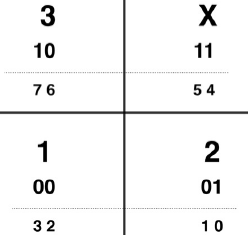
\includegraphics{config2puzzle.png}
\caption{alt}
\end{figure}

Nótese que el orden de los bits que describen las posiciones de cada
casilla se encuentra en un orden invertido que va de derecha a izquierda
y de abajo a arriba. Por ejemlo siendo el orden ABCD, la celda B tiene
las posiciones 2 y 3 solo que se muestra invertido de derecha a
izquierda y se ve como un 3 2.

Comenzamos importando las bibliotecas necesarias e inicializando el
modelo

    \begin{tcolorbox}[breakable, size=fbox, boxrule=1pt, pad at break*=1mm,colback=cellbackground, colframe=cellborder]
\prompt{In}{incolor}{1}{\boxspacing}
\begin{Verbatim}[commandchars=\\\{\}]
\PY{k+kn}{from} \PY{n+nn}{qiskit} \PY{k+kn}{import} \PY{o}{*}
\PY{k+kn}{from} \PY{n+nn}{qiskit}\PY{n+nn}{.}\PY{n+nn}{visualization} \PY{k+kn}{import} \PY{n}{plot\PYZus{}histogram}
\PY{k+kn}{from} \PY{n+nn}{qiskit}\PY{n+nn}{.}\PY{n+nn}{circuit}\PY{n+nn}{.}\PY{n+nn}{library} \PY{k+kn}{import} \PY{n}{MCXGate}
\end{Verbatim}
\end{tcolorbox}

    \begin{tcolorbox}[breakable, size=fbox, boxrule=1pt, pad at break*=1mm,colback=cellbackground, colframe=cellborder]
\prompt{In}{incolor}{2}{\boxspacing}
\begin{Verbatim}[commandchars=\\\{\}]
\PY{k}{def} \PY{n+nf}{posicion\PYZus{}inicial}\PY{p}{(}\PY{n}{qubits\PYZus{}i}\PY{p}{:}\PY{n+nb}{tuple}\PY{p}{)}\PY{p}{:}
    \PY{l+s+sd}{\PYZdq{}\PYZdq{}\PYZdq{}Crea un circuito cuántico de 8 qubits y aplica una compuerta X a los qubits en las posiciones indicadas. }
\PY{l+s+sd}{    El propósito del mismo es representar las posiciones iniciales de las celdas en el puzzle, esto viene a ser el ket x.}
\PY{l+s+sd}{    }
\PY{l+s+sd}{    args}
\PY{l+s+sd}{        qubits\PYZus{}i: En esta tupla de 4 elementos se indican las posiciones de los qubits que serán inicializados como ket 1}
\PY{l+s+sd}{    \PYZdq{}\PYZdq{}\PYZdq{}}
    \PY{n}{qc} \PY{o}{=} \PY{n}{QuantumCircuit}\PY{p}{(}\PY{l+m+mi}{8}\PY{p}{)}
    \PY{c+c1}{\PYZsh{} Preparación de los estados del 0 al 7}
    \PY{n}{qc}\PY{o}{.}\PY{n}{x}\PY{p}{(}\PY{n}{qubits\PYZus{}i}\PY{p}{[}\PY{l+m+mi}{0}\PY{p}{]}\PY{p}{)}
    \PY{n}{qc}\PY{o}{.}\PY{n}{x}\PY{p}{(}\PY{n}{qubits\PYZus{}i}\PY{p}{[}\PY{l+m+mi}{1}\PY{p}{]}\PY{p}{)}
    \PY{n}{qc}\PY{o}{.}\PY{n}{x}\PY{p}{(}\PY{n}{qubits\PYZus{}i}\PY{p}{[}\PY{l+m+mi}{2}\PY{p}{]}\PY{p}{)}
    \PY{n}{qc}\PY{o}{.}\PY{n}{x}\PY{p}{(}\PY{n}{qubits\PYZus{}i}\PY{p}{[}\PY{l+m+mi}{3}\PY{p}{]}\PY{p}{)}
    \PY{n}{qc}\PY{o}{.}\PY{n}{name} \PY{o}{=} \PY{l+s+s2}{\PYZdq{}}\PY{l+s+s2}{init}\PY{l+s+s2}{\PYZdq{}}
    \PY{k}{return} \PY{n}{qc}
\end{Verbatim}
\end{tcolorbox}

    \hypertarget{reglas}{%
\subsection{Reglas}\label{reglas}}

En la tarea de 3 rompecabezas, tenemos cuatro \textbf{reglas} diferentes
definidas por la posición del espacio vacío. Cada una de las reglas
tiene dos instancias, ya sea moviendo el espacio vacío en el sentido de
las agujas del reloj o en el sentido contrario a las agujas del reloj.
Reconocemos las cuatro reglas e indicamos la presencia de una regla
mediante un qubit. Usamos cuatro qubits que indican la presencia de las
cuatro reglas y las llamamos el \textbf{rastro}. Necesitamos el
\textbf{rastro} representado por los cuatro qubits, debido a que no
podemos eliminar la información y no podemos volver a calcular la salida
descomputando rehaceríamos las reglas. Adicionalmente, requerimos una
\textbf{bandera} representada por un qubit que nos indique si la regla
con la instanciación correspondiente se puede ejecutar o no. Finalmente,
necesitamos un qubit que represente el \textbf{descriptor de ruta} que
estará presente por superposición usando una puerta de Hadamard.

En primer lugar, la parte condicional de las reglas es implementada por
la compuerta de Toffoli, llamada también ccx. Reconoce la posición del
espacio vacío y lo indica configurando un qubit de los cuatro qubits del
\emph{rastro} a uno.

    \hypertarget{ejecuciuxf3n-de-las-reglas}{%
\subsection{Ejecución de las
Reglas}\label{ejecuciuxf3n-de-las-reglas}}

La ejecución de las reglas usa la puerta de Fredkin, también llamada
puerta de intercambio controlado (CSWAP), utilizando la información de
seguimiento y el descriptor de ruta configurando el qubit bandera (qubit
8) para indicar si la regla se va a ejecutar. El reinicio se realiza
descomputando, repitiendo la operación para poner la bandera nuevamente
en el estado cero.

Cambiamos el descriptor de la ruta por la puerta NOT y ejecutamos la
segunda instanciación de la regla dependiendo del valor de la traza; el
\texttt{qc.barrier()} separará la representación en el circuito, dando
como resultado el circuito cuántico indicado en la Figura.

    \begin{tcolorbox}[breakable, size=fbox, boxrule=1pt, pad at break*=1mm,colback=cellbackground, colframe=cellborder]
\prompt{In}{incolor}{3}{\boxspacing}
\begin{Verbatim}[commandchars=\\\{\}]
\PY{k}{def} \PY{n+nf}{reglas}\PY{p}{(}\PY{n}{nombre}\PY{p}{:}\PY{n+nb}{str}\PY{p}{,}\PY{n}{tamaño}\PY{p}{:}\PY{n+nb}{int}\PY{p}{,} \PY{n}{bandera}\PY{p}{:}\PY{n+nb}{int}\PY{p}{,} \PY{n}{rastro}\PY{p}{:}\PY{n+nb}{tuple}\PY{p}{,} \PY{n}{descriptor}\PY{p}{:}\PY{n+nb}{int}\PY{p}{)} \PY{o}{\PYZhy{}}\PY{o}{\PYZgt{}} \PY{n}{QuantumCircuit}\PY{p}{:}
    \PY{l+s+sd}{\PYZdq{}\PYZdq{}\PYZdq{}Reglas de movimiento para el 3\PYZhy{}puzzle}
\PY{l+s+sd}{    }
\PY{l+s+sd}{    args}
\PY{l+s+sd}{        nombre: Nombre de las reglas}
\PY{l+s+sd}{        tamaño: El valor define el tamaño del circuito. }
\PY{l+s+sd}{        bandera: (Posición) Indica si la regla puede ejecutarse o no. El valor define la posición de la bandera.}
\PY{l+s+sd}{        rastro: (Posiciones) Cuatro qubits indican la ubicación de la celda vacía. El valor define la posición del rastro.}
\PY{l+s+sd}{        descriptor: (Posición) El descriptor de camino indica el movimiento a realizar. El valor define la posición del descriptor.}
\PY{l+s+sd}{    \PYZdq{}\PYZdq{}\PYZdq{}}
    \PY{n}{qc} \PY{o}{=} \PY{n}{QuantumCircuit}\PY{p}{(}\PY{n}{tamaño}\PY{p}{)}

    \PY{c+c1}{\PYZsh{}If part of rules marked in trace}
    \PY{n}{qc}\PY{o}{.}\PY{n}{ccx}\PY{p}{(}\PY{l+m+mi}{0}\PY{p}{,}\PY{l+m+mi}{1}\PY{p}{,}\PY{n}{rastro}\PY{p}{[}\PY{l+m+mi}{0}\PY{p}{]}\PY{p}{)}
    \PY{n}{qc}\PY{o}{.}\PY{n}{ccx}\PY{p}{(}\PY{l+m+mi}{2}\PY{p}{,}\PY{l+m+mi}{3}\PY{p}{,}\PY{n}{rastro}\PY{p}{[}\PY{l+m+mi}{1}\PY{p}{]}\PY{p}{)}
    \PY{n}{qc}\PY{o}{.}\PY{n}{ccx}\PY{p}{(}\PY{l+m+mi}{4}\PY{p}{,}\PY{l+m+mi}{5}\PY{p}{,}\PY{n}{rastro}\PY{p}{[}\PY{l+m+mi}{2}\PY{p}{]}\PY{p}{)}
    \PY{n}{qc}\PY{o}{.}\PY{n}{ccx}\PY{p}{(}\PY{l+m+mi}{6}\PY{p}{,}\PY{l+m+mi}{7}\PY{p}{,}\PY{n}{rastro}\PY{p}{[}\PY{l+m+mi}{3}\PY{p}{]}\PY{p}{)}
    \PY{n}{qc}\PY{o}{.}\PY{n}{barrier}\PY{p}{(}\PY{p}{)}
    
    \PY{c+c1}{\PYZsh{} Primer conjunto de reglas para la casilla A}

    \PY{c+c1}{\PYZsh{}Search empty state with the descriptor}
    \PY{n}{qc}\PY{o}{.}\PY{n}{ccx}\PY{p}{(}\PY{n}{rastro}\PY{p}{[}\PY{l+m+mi}{0}\PY{p}{]}\PY{p}{,}\PY{n}{descriptor}\PY{p}{,}\PY{n}{bandera}\PY{p}{)}
    \PY{c+c1}{\PYZsh{}Execute 1st then part by moving the empty space anti\PYZhy{}clockwise}
    \PY{n}{qc}\PY{o}{.}\PY{n}{cswap}\PY{p}{(}\PY{n}{bandera}\PY{p}{,}\PY{l+m+mi}{0}\PY{p}{,}\PY{l+m+mi}{4}\PY{p}{)}
    \PY{n}{qc}\PY{o}{.}\PY{n}{cswap}\PY{p}{(}\PY{n}{bandera}\PY{p}{,}\PY{l+m+mi}{1}\PY{p}{,}\PY{l+m+mi}{5}\PY{p}{)}
    \PY{c+c1}{\PYZsh{}Secod then part with changed descriptor}
    \PY{c+c1}{\PYZsh{}Reset Flag}
    \PY{n}{qc}\PY{o}{.}\PY{n}{ccx}\PY{p}{(}\PY{n}{rastro}\PY{p}{[}\PY{l+m+mi}{0}\PY{p}{]}\PY{p}{,}\PY{n}{descriptor}\PY{p}{,}\PY{n}{bandera}\PY{p}{)}
    \PY{c+c1}{\PYZsh{}Fetch second superposition}
    \PY{n}{qc}\PY{o}{.}\PY{n}{x}\PY{p}{(}\PY{n}{descriptor}\PY{p}{)}
    \PY{n}{qc}\PY{o}{.}\PY{n}{ccx}\PY{p}{(}\PY{n}{rastro}\PY{p}{[}\PY{l+m+mi}{0}\PY{p}{]}\PY{p}{,}\PY{n}{descriptor}\PY{p}{,}\PY{n}{bandera}\PY{p}{)}
    \PY{c+c1}{\PYZsh{}Execute 2th then part by moving the empty space clockwise}
    \PY{n}{qc}\PY{o}{.}\PY{n}{cswap}\PY{p}{(}\PY{n}{bandera}\PY{p}{,}\PY{l+m+mi}{0}\PY{p}{,}\PY{l+m+mi}{2}\PY{p}{)}
    \PY{n}{qc}\PY{o}{.}\PY{n}{cswap}\PY{p}{(}\PY{n}{bandera}\PY{p}{,}\PY{l+m+mi}{1}\PY{p}{,}\PY{l+m+mi}{3}\PY{p}{)}
    \PY{c+c1}{\PYZsh{}Reset Flag}
    \PY{n}{qc}\PY{o}{.}\PY{n}{ccx}\PY{p}{(}\PY{n}{rastro}\PY{p}{[}\PY{l+m+mi}{0}\PY{p}{]}\PY{p}{,}\PY{n}{descriptor}\PY{p}{,}\PY{n}{bandera}\PY{p}{)}
    \PY{c+c1}{\PYZsh{}Restore descriptor}
    \PY{n}{qc}\PY{o}{.}\PY{n}{x}\PY{p}{(}\PY{n}{descriptor}\PY{p}{)}
    \PY{n}{qc}\PY{o}{.}\PY{n}{barrier}\PY{p}{(}\PY{p}{)}

    \PY{c+c1}{\PYZsh{} Segundo conjunto de reglas para la casilla B}

    \PY{c+c1}{\PYZsh{}Search empty state with the descriptor}
    \PY{n}{qc}\PY{o}{.}\PY{n}{ccx}\PY{p}{(}\PY{n}{rastro}\PY{p}{[}\PY{l+m+mi}{1}\PY{p}{]}\PY{p}{,}\PY{n}{descriptor}\PY{p}{,}\PY{n}{bandera}\PY{p}{)}
    \PY{c+c1}{\PYZsh{}Execute 1st then part}
    \PY{n}{qc}\PY{o}{.}\PY{n}{cswap}\PY{p}{(}\PY{n}{bandera}\PY{p}{,}\PY{l+m+mi}{0}\PY{p}{,}\PY{l+m+mi}{2}\PY{p}{)}
    \PY{n}{qc}\PY{o}{.}\PY{n}{cswap}\PY{p}{(}\PY{n}{bandera}\PY{p}{,}\PY{l+m+mi}{1}\PY{p}{,}\PY{l+m+mi}{3}\PY{p}{)}
    \PY{c+c1}{\PYZsh{}Secod then part with changed descriptor}
    \PY{c+c1}{\PYZsh{}Reset Flag}
    \PY{n}{qc}\PY{o}{.}\PY{n}{ccx}\PY{p}{(}\PY{n}{rastro}\PY{p}{[}\PY{l+m+mi}{1}\PY{p}{]}\PY{p}{,}\PY{n}{descriptor}\PY{p}{,}\PY{n}{bandera}\PY{p}{)}
    \PY{c+c1}{\PYZsh{}Fetch second superposition}
    \PY{n}{qc}\PY{o}{.}\PY{n}{x}\PY{p}{(}\PY{n}{descriptor}\PY{p}{)}
    \PY{n}{qc}\PY{o}{.}\PY{n}{ccx}\PY{p}{(}\PY{n}{rastro}\PY{p}{[}\PY{l+m+mi}{1}\PY{p}{]}\PY{p}{,}\PY{n}{descriptor}\PY{p}{,}\PY{n}{bandera}\PY{p}{)}
    \PY{c+c1}{\PYZsh{}Execute 2th then part}
    \PY{n}{qc}\PY{o}{.}\PY{n}{cswap}\PY{p}{(}\PY{n}{bandera}\PY{p}{,}\PY{l+m+mi}{2}\PY{p}{,}\PY{l+m+mi}{6}\PY{p}{)}
    \PY{n}{qc}\PY{o}{.}\PY{n}{cswap}\PY{p}{(}\PY{n}{bandera}\PY{p}{,}\PY{l+m+mi}{3}\PY{p}{,}\PY{l+m+mi}{7}\PY{p}{)}
    \PY{c+c1}{\PYZsh{}Reset Flag}
    \PY{n}{qc}\PY{o}{.}\PY{n}{ccx}\PY{p}{(}\PY{n}{rastro}\PY{p}{[}\PY{l+m+mi}{1}\PY{p}{]}\PY{p}{,}\PY{n}{descriptor}\PY{p}{,}\PY{n}{bandera}\PY{p}{)}
    \PY{c+c1}{\PYZsh{}Restore descriptor}
    \PY{n}{qc}\PY{o}{.}\PY{n}{x}\PY{p}{(}\PY{n}{descriptor}\PY{p}{)}
    \PY{n}{qc}\PY{o}{.}\PY{n}{barrier}\PY{p}{(}\PY{p}{)}

    \PY{c+c1}{\PYZsh{} Tercer conjunto de reglas para la casilla C}

    \PY{c+c1}{\PYZsh{}Search empty state with the descriptor}
    \PY{n}{qc}\PY{o}{.}\PY{n}{ccx}\PY{p}{(}\PY{n}{rastro}\PY{p}{[}\PY{l+m+mi}{2}\PY{p}{]}\PY{p}{,}\PY{n}{descriptor}\PY{p}{,}\PY{n}{bandera}\PY{p}{)}
    \PY{c+c1}{\PYZsh{}Execute 1st then part}
    \PY{n}{qc}\PY{o}{.}\PY{n}{cswap}\PY{p}{(}\PY{n}{bandera}\PY{p}{,}\PY{l+m+mi}{4}\PY{p}{,}\PY{l+m+mi}{6}\PY{p}{)}
    \PY{n}{qc}\PY{o}{.}\PY{n}{cswap}\PY{p}{(}\PY{n}{bandera}\PY{p}{,}\PY{l+m+mi}{5}\PY{p}{,}\PY{l+m+mi}{7}\PY{p}{)}
    \PY{c+c1}{\PYZsh{}Secod then part with changed descriptor}
    \PY{c+c1}{\PYZsh{}Reset Flag}
    \PY{n}{qc}\PY{o}{.}\PY{n}{ccx}\PY{p}{(}\PY{n}{rastro}\PY{p}{[}\PY{l+m+mi}{2}\PY{p}{]}\PY{p}{,}\PY{n}{descriptor}\PY{p}{,}\PY{n}{bandera}\PY{p}{)}
    \PY{c+c1}{\PYZsh{}Fetch second superposition}
    \PY{n}{qc}\PY{o}{.}\PY{n}{x}\PY{p}{(}\PY{n}{descriptor}\PY{p}{)}
    \PY{n}{qc}\PY{o}{.}\PY{n}{ccx}\PY{p}{(}\PY{n}{rastro}\PY{p}{[}\PY{l+m+mi}{2}\PY{p}{]}\PY{p}{,}\PY{n}{descriptor}\PY{p}{,}\PY{n}{bandera}\PY{p}{)}
    \PY{c+c1}{\PYZsh{}Execute 2th then part}
    \PY{n}{qc}\PY{o}{.}\PY{n}{cswap}\PY{p}{(}\PY{n}{bandera}\PY{p}{,}\PY{l+m+mi}{0}\PY{p}{,}\PY{l+m+mi}{4}\PY{p}{)}
    \PY{n}{qc}\PY{o}{.}\PY{n}{cswap}\PY{p}{(}\PY{n}{bandera}\PY{p}{,}\PY{l+m+mi}{1}\PY{p}{,}\PY{l+m+mi}{5}\PY{p}{)}
    \PY{c+c1}{\PYZsh{}Reset Flag}
    \PY{n}{qc}\PY{o}{.}\PY{n}{ccx}\PY{p}{(}\PY{n}{rastro}\PY{p}{[}\PY{l+m+mi}{2}\PY{p}{]}\PY{p}{,}\PY{n}{descriptor}\PY{p}{,}\PY{n}{bandera}\PY{p}{)}
    \PY{c+c1}{\PYZsh{}Restore descriptor}
    \PY{n}{qc}\PY{o}{.}\PY{n}{x}\PY{p}{(}\PY{n}{descriptor}\PY{p}{)}
    \PY{n}{qc}\PY{o}{.}\PY{n}{barrier}\PY{p}{(}\PY{p}{)}

    \PY{c+c1}{\PYZsh{} Cuarto conjunto de reglas para la casilla D}

    \PY{c+c1}{\PYZsh{}Search empty state with the descriptor}
    \PY{n}{qc}\PY{o}{.}\PY{n}{ccx}\PY{p}{(}\PY{n}{rastro}\PY{p}{[}\PY{l+m+mi}{3}\PY{p}{]}\PY{p}{,}\PY{n}{descriptor}\PY{p}{,}\PY{n}{bandera}\PY{p}{)}
    \PY{c+c1}{\PYZsh{}Execute 1st then part}
    \PY{n}{qc}\PY{o}{.}\PY{n}{cswap}\PY{p}{(}\PY{n}{bandera}\PY{p}{,}\PY{l+m+mi}{2}\PY{p}{,}\PY{l+m+mi}{6}\PY{p}{)}
    \PY{n}{qc}\PY{o}{.}\PY{n}{cswap}\PY{p}{(}\PY{n}{bandera}\PY{p}{,}\PY{l+m+mi}{3}\PY{p}{,}\PY{l+m+mi}{7}\PY{p}{)}
    \PY{c+c1}{\PYZsh{}Secod then part with changed descriptor}
    \PY{c+c1}{\PYZsh{}Reset Flag}
    \PY{n}{qc}\PY{o}{.}\PY{n}{ccx}\PY{p}{(}\PY{n}{rastro}\PY{p}{[}\PY{l+m+mi}{3}\PY{p}{]}\PY{p}{,}\PY{n}{descriptor}\PY{p}{,}\PY{n}{bandera}\PY{p}{)}
    \PY{c+c1}{\PYZsh{}Fetch second superposition}
    \PY{n}{qc}\PY{o}{.}\PY{n}{x}\PY{p}{(}\PY{n}{descriptor}\PY{p}{)}
    \PY{n}{qc}\PY{o}{.}\PY{n}{ccx}\PY{p}{(}\PY{n}{rastro}\PY{p}{[}\PY{l+m+mi}{3}\PY{p}{]}\PY{p}{,}\PY{n}{descriptor}\PY{p}{,}\PY{n}{bandera}\PY{p}{)}
    \PY{c+c1}{\PYZsh{}Execute 2th then part}
    \PY{n}{qc}\PY{o}{.}\PY{n}{cswap}\PY{p}{(}\PY{n}{bandera}\PY{p}{,}\PY{l+m+mi}{4}\PY{p}{,}\PY{l+m+mi}{6}\PY{p}{)}
    \PY{n}{qc}\PY{o}{.}\PY{n}{cswap}\PY{p}{(}\PY{n}{bandera}\PY{p}{,}\PY{l+m+mi}{5}\PY{p}{,}\PY{l+m+mi}{7}\PY{p}{)}
    \PY{c+c1}{\PYZsh{}Reset Flag}
    \PY{n}{qc}\PY{o}{.}\PY{n}{ccx}\PY{p}{(}\PY{n}{rastro}\PY{p}{[}\PY{l+m+mi}{3}\PY{p}{]}\PY{p}{,}\PY{n}{descriptor}\PY{p}{,}\PY{n}{bandera}\PY{p}{)}
    \PY{c+c1}{\PYZsh{}Restore descriptor}
    \PY{n}{qc}\PY{o}{.}\PY{n}{x}\PY{p}{(}\PY{n}{descriptor}\PY{p}{)}
    \PY{n}{qc}\PY{o}{.}\PY{n}{barrier}\PY{p}{(}\PY{p}{)}
    \PY{n}{qc}\PY{o}{.}\PY{n}{name} \PY{o}{=} \PY{n}{nombre}
    
    \PY{c+c1}{\PYZsh{} Se muestra la estructura del circuito en caso de querer visualizarla}
    \PY{k}{if} \PY{n}{nombre} \PY{o}{==} \PY{l+s+s1}{\PYZsq{}}\PY{l+s+s1}{test}\PY{l+s+s1}{\PYZsq{}}\PY{p}{:}
        \PY{n}{display}\PY{p}{(}
            \PY{n}{qc}\PY{o}{.}\PY{n}{draw}\PY{p}{(}\PY{n}{output}\PY{o}{=}\PY{l+s+s1}{\PYZsq{}}\PY{l+s+s1}{mpl}\PY{l+s+s1}{\PYZsq{}}\PY{p}{,} \PY{n}{fold}\PY{o}{=}\PY{o}{\PYZhy{}}\PY{l+m+mi}{1}\PY{p}{)}
        \PY{p}{)}
    \PY{k}{return} \PY{n}{qc}

\PY{n}{reglas}\PY{p}{(}\PY{n}{nombre}\PY{o}{=}\PY{l+s+s2}{\PYZdq{}}\PY{l+s+s2}{test}\PY{l+s+s2}{\PYZdq{}}\PY{p}{,}\PY{n}{tamaño}\PY{o}{=}\PY{l+m+mi}{14}\PY{p}{,}\PY{n}{bandera}\PY{o}{=}\PY{l+m+mi}{8}\PY{p}{,}\PY{n}{rastro}\PY{o}{=}\PY{p}{(}\PY{l+m+mi}{9}\PY{p}{,}\PY{l+m+mi}{10}\PY{p}{,}\PY{l+m+mi}{11}\PY{p}{,}\PY{l+m+mi}{12}\PY{p}{)}\PY{p}{,}\PY{n}{descriptor}\PY{o}{=}\PY{l+m+mi}{13}\PY{p}{)}
\end{Verbatim}
\end{tcolorbox}

    \begin{center}
    \adjustimage{max size={0.9\linewidth}{0.9\paperheight}}{qtree_files/qtree_7_0.png}
    \end{center}
    { \hspace*{\fill} \\}
    
            \begin{tcolorbox}[breakable, size=fbox, boxrule=.5pt, pad at break*=1mm, opacityfill=0]
\prompt{Out}{outcolor}{3}{\boxspacing}
\begin{Verbatim}[commandchars=\\\{\}]
<qiskit.circuit.quantumcircuit.QuantumCircuit at 0x283d1466ec0>
\end{Verbatim}
\end{tcolorbox}
        
    \hypertarget{profundidad-2}{%
\section{3-puzzle de profundidad 2}\label{profundidad-2}}

La amplificación de Grover no se puede aplicar a menos de cuatro
estados. Una búsqueda de profundidad uno para el rompecabezas de 3 parte
los resultados en dos estados y una búsqueda de profundidad dos en
cuatro estados. El operador \(L(2)\) que describe la búsqueda de la
profundidad dos se representa como

\(L(2) \ket{m_2 , m_1}\ket{x} = \ket{m_2 , m_1}\ket{\gamma}\)

con dos qubits representando el camino que tomará.

El operador \(T\) representa la función oráculo. La cual sirve para
verificar si se ha alcanzado la solución.

Con búsqueda en profundidad \(t = 2\), se necesitan cuatro qubits
adicionales para representar la nueva traza, un qubit adicional para el
descriptor de ruta de la profundidad dos y un qubit auxiliar para la
operación del oráculo. El circuito cuántico para este caso está
representado por 20 qubits. Medimos el descriptor de ruta representado
por dos qubits 13 y 18.

En el ejemplo siguiente las variables init y goal definen la
configuración inicial de las celdas del puzzle y la configuración
objetivo, La siguiente imagen representa la posición inicial de las
celdas en las configuraciones indicadas en el código.

\begin{figure}
\centering
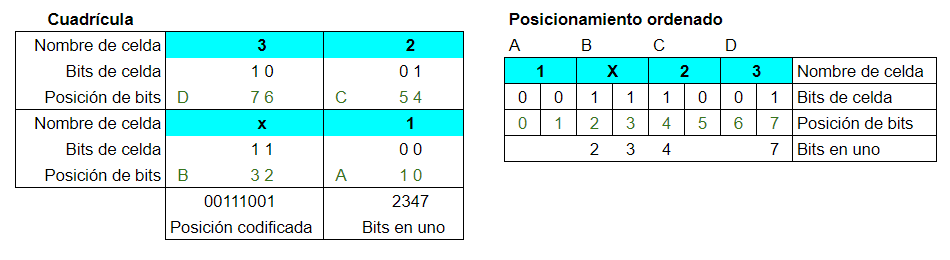
\includegraphics{Posicion-inicial.png}
\caption{alt}
\end{figure}

La posición de los bits en 1 del registro de las cuatro celdas (los 8
bits que definen la posición de las celdas) es lo que define la
configuración inicial y objetivo del puzzle. En este caso la
configuración inicial es 2-3-4-7, y la objetivo es 0-4-5-7 la cual es
llevar la celda vacía hasta la posición C en sentido antihorario.

\begin{figure}
\centering
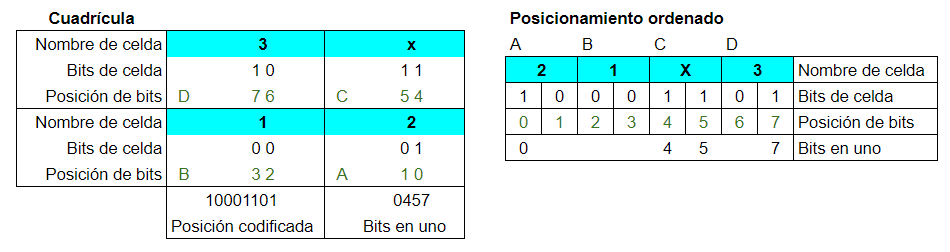
\includegraphics{Posicion-final1.png}
\caption{alt}
\end{figure}

    \begin{tcolorbox}[breakable, size=fbox, boxrule=1pt, pad at break*=1mm,colback=cellbackground, colframe=cellborder]
\prompt{In}{incolor}{4}{\boxspacing}
\begin{Verbatim}[commandchars=\\\{\}]
\PY{k}{def} \PY{n+nf}{oracle}\PY{p}{(}\PY{n}{size}\PY{p}{:}\PY{n+nb}{int}\PY{p}{,} \PY{n}{qubits\PYZus{}t}\PY{p}{:}\PY{n+nb}{tuple}\PY{p}{)}\PY{p}{:}
    \PY{l+s+sd}{\PYZdq{}\PYZdq{}\PYZdq{}Oráculo. Verifica si se ha alcanzado la solución.}
\PY{l+s+sd}{    }
\PY{l+s+sd}{    args}
\PY{l+s+sd}{        size: El tamaño en qubits del circuito}
\PY{l+s+sd}{        qubits\PYZus{}t: Esta tupla define la solución (target) del puzzle por la posición de los qubits en 1.}
\PY{l+s+sd}{    \PYZdq{}\PYZdq{}\PYZdq{}}
    \PY{n}{qc} \PY{o}{=} \PY{n}{QuantumCircuit}\PY{p}{(}\PY{n}{size}\PY{p}{)}
    \PY{n}{gate} \PY{o}{=} \PY{n}{MCXGate}\PY{p}{(}\PY{l+m+mi}{4}\PY{p}{)}
    \PY{c+c1}{\PYZsh{}Goal Configurations}
    \PY{n}{qc}\PY{o}{.}\PY{n}{append}\PY{p}{(}\PY{n}{gate}\PY{p}{,}\PY{p}{[}\PY{n}{qubits\PYZus{}t}\PY{p}{[}\PY{l+m+mi}{0}\PY{p}{]}\PY{p}{,} \PY{n}{qubits\PYZus{}t}\PY{p}{[}\PY{l+m+mi}{1}\PY{p}{]}\PY{p}{,} \PY{n}{qubits\PYZus{}t}\PY{p}{[}\PY{l+m+mi}{2}\PY{p}{]}\PY{p}{,} \PY{n}{qubits\PYZus{}t}\PY{p}{[}\PY{l+m+mi}{3}\PY{p}{]}\PY{p}{,} \PY{n}{size}\PY{o}{\PYZhy{}}\PY{l+m+mi}{1}\PY{p}{]}\PY{p}{)}
    \PY{n}{qc}\PY{o}{.}\PY{n}{name}\PY{o}{=}\PY{l+s+s2}{\PYZdq{}}\PY{l+s+s2}{ Orac}\PY{l+s+s2}{\PYZdq{}}
    \PY{k}{return} \PY{n}{qc}
    
\PY{k}{def} \PY{n+nf}{reglas\PYZus{}inv}\PY{p}{(}\PY{n}{nombre}\PY{p}{:}\PY{n+nb}{str}\PY{p}{,} \PY{n}{tamaño}\PY{p}{:}\PY{n+nb}{int}\PY{p}{,} \PY{n}{bandera}\PY{p}{:}\PY{n+nb}{int}\PY{p}{,} \PY{n}{rastro}\PY{p}{:}\PY{n+nb}{tuple}\PY{p}{,} \PY{n}{descriptor}\PY{p}{:}\PY{n+nb}{int}\PY{p}{)} \PY{o}{\PYZhy{}}\PY{o}{\PYZgt{}} \PY{n}{QuantumCircuit}\PY{p}{:}
    \PY{n}{qc} \PY{o}{=} \PY{n}{reglas}\PY{p}{(}\PY{n}{nombre}\PY{p}{,} \PY{n}{tamaño}\PY{p}{,} \PY{n}{bandera}\PY{p}{,} \PY{n}{rastro}\PY{p}{,} \PY{n}{descriptor}\PY{p}{)}
    \PY{n}{qc\PYZus{}inv} \PY{o}{=} \PY{n}{qc}\PY{o}{.}\PY{n}{inverse}\PY{p}{(}\PY{p}{)}
    \PY{n}{qc\PYZus{}inv}\PY{o}{.}\PY{n}{name} \PY{o}{=} \PY{n}{nombre} \PY{o}{+} \PY{l+s+s2}{\PYZdq{}}\PY{l+s+s2}{\PYZus{}inv}\PY{l+s+s2}{\PYZdq{}}
    \PY{k}{return} \PY{n}{qc\PYZus{}inv}

\PY{k}{def} \PY{n+nf}{Grover}\PY{p}{(}\PY{p}{)}\PY{p}{:}
    \PY{l+s+sd}{\PYZdq{}\PYZdq{}\PYZdq{}Grover para el caso de profundidad 2\PYZdq{}\PYZdq{}\PYZdq{}}
    \PY{n}{qc} \PY{o}{=} \PY{n}{QuantumCircuit}\PY{p}{(}\PY{l+m+mi}{19}\PY{p}{)}
    \PY{c+c1}{\PYZsh{}Diffusor}
    \PY{n}{qc}\PY{o}{.}\PY{n}{h}\PY{p}{(}\PY{p}{[}\PY{l+m+mi}{13}\PY{p}{,}\PY{l+m+mi}{18}\PY{p}{]}\PY{p}{)}
    \PY{n}{qc}\PY{o}{.}\PY{n}{z}\PY{p}{(}\PY{p}{[}\PY{l+m+mi}{13}\PY{p}{,}\PY{l+m+mi}{18}\PY{p}{]}\PY{p}{)}
    \PY{n}{qc}\PY{o}{.}\PY{n}{cz}\PY{p}{(}\PY{l+m+mi}{13}\PY{p}{,}\PY{l+m+mi}{18}\PY{p}{)}
    \PY{n}{qc}\PY{o}{.}\PY{n}{h}\PY{p}{(}\PY{p}{[}\PY{l+m+mi}{13}\PY{p}{,}\PY{l+m+mi}{18}\PY{p}{]}\PY{p}{)}
    \PY{n}{qc}\PY{o}{.}\PY{n}{name}\PY{o}{=}\PY{l+s+s2}{\PYZdq{}}\PY{l+s+s2}{G}\PY{l+s+s2}{\PYZdq{}}
    \PY{k}{return} \PY{n}{qc}
    
\PY{c+c1}{\PYZsh{} Inicialización del circuito cuántico con 25 qubits.}
\PY{n}{qc2} \PY{o}{=} \PY{n}{QuantumCircuit}\PY{p}{(}\PY{l+m+mi}{20}\PY{p}{,}\PY{l+m+mi}{2}\PY{p}{)}
\PY{c+c1}{\PYZsh{} Posición de las celdas inicial y final, descritas como la posición de los qubits que son ket 1}
\PY{n}{init} \PY{o}{=} \PY{p}{(}\PY{l+m+mi}{2}\PY{p}{,}\PY{l+m+mi}{3}\PY{p}{,}\PY{l+m+mi}{4}\PY{p}{,}\PY{l+m+mi}{7}\PY{p}{)}
\PY{n}{goal} \PY{o}{=} \PY{p}{(}\PY{l+m+mi}{0}\PY{p}{,}\PY{l+m+mi}{4}\PY{p}{,}\PY{l+m+mi}{5}\PY{p}{,}\PY{l+m+mi}{7}\PY{p}{)}
\PY{c+c1}{\PYZsh{} Colocamos en superposición los descriptores de camino 13, 18 y 23}
\PY{n}{qc2}\PY{o}{.}\PY{n}{h}\PY{p}{(}\PY{l+m+mi}{13}\PY{p}{)}
\PY{n}{qc2}\PY{o}{.}\PY{n}{h}\PY{p}{(}\PY{l+m+mi}{18}\PY{p}{)}

\PY{c+c1}{\PYZsh{} Qubit auxiliar que indica si se alcanzó la solución, se niega y se coloca en superposición}
\PY{n}{qc2}\PY{o}{.}\PY{n}{x}\PY{p}{(}\PY{l+m+mi}{19}\PY{p}{)}
\PY{n}{qc2}\PY{o}{.}\PY{n}{h}\PY{p}{(}\PY{l+m+mi}{19}\PY{p}{)}
\PY{n}{qc2}\PY{o}{.}\PY{n}{barrier}\PY{p}{(}\PY{p}{)}

\PY{c+c1}{\PYZsh{} Preparación del estado inicial}
\PY{n}{qc2}\PY{o}{.}\PY{n}{append}\PY{p}{(}\PY{n}{posicion\PYZus{}inicial}\PY{p}{(}\PY{n}{init}\PY{p}{)}\PY{p}{,}\PY{n+nb}{range}\PY{p}{(}\PY{l+m+mi}{8}\PY{p}{)}\PY{p}{)}
\PY{n}{qc2}\PY{o}{.}\PY{n}{append}\PY{p}{(}\PY{n}{reglas}\PY{p}{(}\PY{n}{nombre}\PY{o}{=}\PY{l+s+s2}{\PYZdq{}}\PY{l+s+s2}{Reglas1}\PY{l+s+s2}{\PYZdq{}}\PY{p}{,}\PY{n}{tamaño}\PY{o}{=}\PY{l+m+mi}{14}\PY{p}{,}\PY{n}{bandera}\PY{o}{=}\PY{l+m+mi}{8}\PY{p}{,} \PY{n}{rastro}\PY{o}{=}\PY{p}{(}\PY{l+m+mi}{9}\PY{p}{,}\PY{l+m+mi}{10}\PY{p}{,}\PY{l+m+mi}{11}\PY{p}{,}\PY{l+m+mi}{12}\PY{p}{)}\PY{p}{,}\PY{n}{descriptor}\PY{o}{=}\PY{l+m+mi}{13}\PY{p}{)}\PY{p}{,} \PY{n+nb}{range}\PY{p}{(}\PY{l+m+mi}{14}\PY{p}{)}\PY{p}{)}
\PY{n}{qc2}\PY{o}{.}\PY{n}{append}\PY{p}{(}\PY{n}{reglas}\PY{p}{(}\PY{n}{nombre}\PY{o}{=}\PY{l+s+s2}{\PYZdq{}}\PY{l+s+s2}{Reglas2}\PY{l+s+s2}{\PYZdq{}}\PY{p}{,}\PY{n}{tamaño}\PY{o}{=}\PY{l+m+mi}{19}\PY{p}{,}\PY{n}{bandera}\PY{o}{=}\PY{l+m+mi}{8}\PY{p}{,} \PY{n}{rastro}\PY{o}{=}\PY{p}{(}\PY{l+m+mi}{14}\PY{p}{,}\PY{l+m+mi}{15}\PY{p}{,}\PY{l+m+mi}{16}\PY{p}{,}\PY{l+m+mi}{17}\PY{p}{)}\PY{p}{,}\PY{n}{descriptor}\PY{o}{=}\PY{l+m+mi}{18}\PY{p}{)}\PY{p}{,}\PY{n+nb}{range}\PY{p}{(}\PY{l+m+mi}{19}\PY{p}{)}\PY{p}{)}
\PY{c+c1}{\PYZsh{} Oráculo}
\PY{n}{qc2}\PY{o}{.}\PY{n}{append}\PY{p}{(}\PY{n}{oracle}\PY{p}{(}\PY{l+m+mi}{20}\PY{p}{,} \PY{n}{goal}\PY{p}{)}\PY{p}{,}\PY{n+nb}{range}\PY{p}{(}\PY{l+m+mi}{20}\PY{p}{)}\PY{p}{)}
\PY{n}{qc2}\PY{o}{.}\PY{n}{append}\PY{p}{(}\PY{n}{reglas\PYZus{}inv}\PY{p}{(}\PY{n}{nombre}\PY{o}{=}\PY{l+s+s2}{\PYZdq{}}\PY{l+s+s2}{Reglas2}\PY{l+s+s2}{\PYZdq{}}\PY{p}{,}\PY{n}{tamaño}\PY{o}{=}\PY{l+m+mi}{19}\PY{p}{,}\PY{n}{bandera}\PY{o}{=}\PY{l+m+mi}{8}\PY{p}{,} \PY{n}{rastro}\PY{o}{=}\PY{p}{(}\PY{l+m+mi}{14}\PY{p}{,}\PY{l+m+mi}{15}\PY{p}{,}\PY{l+m+mi}{16}\PY{p}{,}\PY{l+m+mi}{17}\PY{p}{)}\PY{p}{,}\PY{n}{descriptor}\PY{o}{=}\PY{l+m+mi}{18}\PY{p}{)}\PY{p}{,}\PY{n+nb}{range}\PY{p}{(}\PY{l+m+mi}{19}\PY{p}{)}\PY{p}{)}
\PY{n}{qc2}\PY{o}{.}\PY{n}{append}\PY{p}{(}\PY{n}{reglas\PYZus{}inv}\PY{p}{(}\PY{n}{nombre}\PY{o}{=}\PY{l+s+s2}{\PYZdq{}}\PY{l+s+s2}{Reglas1}\PY{l+s+s2}{\PYZdq{}}\PY{p}{,}\PY{n}{tamaño}\PY{o}{=}\PY{l+m+mi}{14}\PY{p}{,}\PY{n}{bandera}\PY{o}{=}\PY{l+m+mi}{8}\PY{p}{,} \PY{n}{rastro}\PY{o}{=}\PY{p}{(}\PY{l+m+mi}{9}\PY{p}{,}\PY{l+m+mi}{10}\PY{p}{,}\PY{l+m+mi}{11}\PY{p}{,}\PY{l+m+mi}{12}\PY{p}{)}\PY{p}{,}\PY{n}{descriptor}\PY{o}{=}\PY{l+m+mi}{13}\PY{p}{)}\PY{p}{,} \PY{n+nb}{range}\PY{p}{(}\PY{l+m+mi}{14}\PY{p}{)}\PY{p}{)}
\PY{c+c1}{\PYZsh{} Rehacemos la preparación}
\PY{n}{qc2}\PY{o}{.}\PY{n}{append}\PY{p}{(}\PY{n}{posicion\PYZus{}inicial}\PY{p}{(}\PY{n}{init}\PY{p}{)}\PY{p}{,}\PY{n+nb}{range}\PY{p}{(}\PY{l+m+mi}{8}\PY{p}{)}\PY{p}{)}
\PY{n}{qc2}\PY{o}{.}\PY{n}{barrier}\PY{p}{(}\PY{p}{)}
\PY{c+c1}{\PYZsh{} Rehacemos la superposición del qubit auxiliar}
\PY{n}{qc2}\PY{o}{.}\PY{n}{h}\PY{p}{(}\PY{l+m+mi}{19}\PY{p}{)}
\PY{n}{qc2}\PY{o}{.}\PY{n}{barrier}\PY{p}{(}\PY{p}{)}
\PY{n}{qc2}\PY{o}{.}\PY{n}{append}\PY{p}{(}\PY{n}{Grover}\PY{p}{(}\PY{p}{)}\PY{p}{,}\PY{n+nb}{range}\PY{p}{(}\PY{l+m+mi}{19}\PY{p}{)}\PY{p}{)}
\PY{n}{qc2}\PY{o}{.}\PY{n}{measure}\PY{p}{(}\PY{l+m+mi}{13}\PY{p}{,}\PY{l+m+mi}{0}\PY{p}{)}
\PY{n}{qc2}\PY{o}{.}\PY{n}{measure}\PY{p}{(}\PY{l+m+mi}{18}\PY{p}{,}\PY{l+m+mi}{1}\PY{p}{)}


\PY{c+c1}{\PYZsh{} Visualización del circuito}
\PY{n}{estilo} \PY{o}{=} \PY{p}{\PYZob{}} \PY{l+s+s2}{\PYZdq{}}\PY{l+s+s2}{displaycolor}\PY{l+s+s2}{\PYZdq{}}\PY{p}{:} \PY{p}{\PYZob{}} \PY{l+s+s2}{\PYZdq{}}\PY{l+s+s2}{ Orac}\PY{l+s+s2}{\PYZdq{}}\PY{p}{:} \PY{p}{[}\PY{l+s+s2}{\PYZdq{}}\PY{l+s+s2}{\PYZsh{}03D08C}\PY{l+s+s2}{\PYZdq{}}\PY{p}{,} \PY{l+s+s2}{\PYZdq{}}\PY{l+s+s2}{\PYZsh{}000000}\PY{l+s+s2}{\PYZdq{}}\PY{p}{]} \PY{p}{\PYZcb{}} \PY{p}{\PYZcb{}}
\PY{n}{display}\PY{p}{(}
    \PY{n}{qc2}\PY{o}{.}\PY{n}{draw}\PY{p}{(}\PY{n}{output}\PY{o}{=}\PY{l+s+s1}{\PYZsq{}}\PY{l+s+s1}{mpl}\PY{l+s+s1}{\PYZsq{}}\PY{p}{,} \PY{n}{style}\PY{o}{=}\PY{n}{estilo}\PY{p}{)}
\PY{p}{)}
\end{Verbatim}
\end{tcolorbox}

    \begin{center}
    \adjustimage{max size={0.9\linewidth}{0.9\paperheight}}{qtree_files/qtree_9_0.png}
    \end{center}
    { \hspace*{\fill} \\}
    
    Se puede apreciar en la gráfica que la solución para este caso es 11, es
decir mover la casilla en sentido horario dos veces.

    \begin{tcolorbox}[breakable, size=fbox, boxrule=1pt, pad at break*=1mm,colback=cellbackground, colframe=cellborder]
\prompt{In}{incolor}{5}{\boxspacing}
\begin{Verbatim}[commandchars=\\\{\}]
\PY{c+c1}{\PYZsh{} Simulador }
\PY{n}{simulator2} \PY{o}{=} \PY{n}{Aer}\PY{o}{.}\PY{n}{get\PYZus{}backend}\PY{p}{(}\PY{l+s+s1}{\PYZsq{}}\PY{l+s+s1}{qasm\PYZus{}simulator}\PY{l+s+s1}{\PYZsq{}}\PY{p}{)}
\PY{n}{result2}\PY{o}{=}\PY{n}{execute}\PY{p}{(}\PY{n}{qc2}\PY{p}{,}\PY{n}{simulator2}\PY{p}{,} \PY{n}{shots}\PY{o}{=}\PY{l+m+mi}{512}\PY{p}{)}\PY{o}{.}\PY{n}{result}\PY{p}{(}\PY{p}{)}
\PY{n}{counts2} \PY{o}{=} \PY{n}{result2}\PY{o}{.}\PY{n}{get\PYZus{}counts}\PY{p}{(}\PY{p}{)}
\PY{n}{plot\PYZus{}histogram}\PY{p}{(}\PY{n}{counts2}\PY{p}{)}
\end{Verbatim}
\end{tcolorbox}
 
            
\prompt{Out}{outcolor}{5}{}
    
    \begin{center}
    \adjustimage{max size={0.9\linewidth}{0.9\paperheight}}{qtree_files/qtree_11_0.png}
    \end{center}
    { \hspace*{\fill} \\}
    

    \hypertarget{profundidad-3}{%
\section{3-puzzle de profundidad 3}\label{profundidad-3}}

Este caso es similar a los anteriores aunque el Grover es diferente.

En este ejemplo nuevamente las variables init y goal definen la
configuración inicial de las celdas del puzzle y la configuración
objetivo, esta vez la configuración objetivo por tratarse de 3
movimientos existen tres maneras de llegar a la configuración objetivo.

\hypertarget{configuraciuxf3n-inicial-y-final}{%
\paragraph{Configuración inicial y
final}\label{configuraciuxf3n-inicial-y-final}}

La configuración inicial es la misma que en el caso anterior 2-3-4-7,
sin embargo la configuración final para este caso es 0-1-4-7, la cual
puede apreciarse en la figura siguiente.

\begin{figure}
\centering
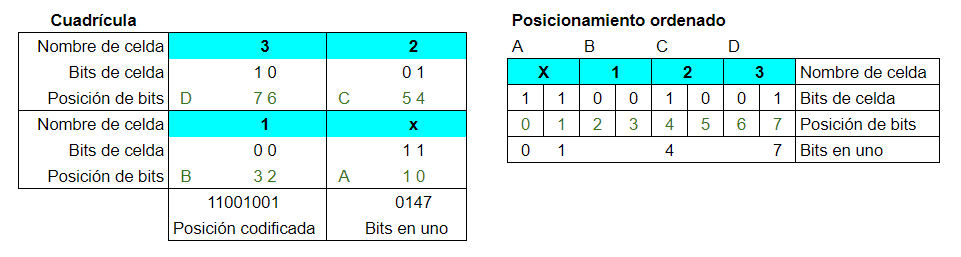
\includegraphics{Posicion-final2.png}
\caption{alt}
\end{figure}

Nótese que la solución se puede hallar con un solo movimiento al mover
la celda vacía a la derecha, sin embargo en este caso se requiere una
solución que consista estrictamente de tres movimientos.

    \begin{tcolorbox}[breakable, size=fbox, boxrule=1pt, pad at break*=1mm,colback=cellbackground, colframe=cellborder]
\prompt{In}{incolor}{8}{\boxspacing}
\begin{Verbatim}[commandchars=\\\{\}]
\PY{k}{def} \PY{n+nf}{Grover3}\PY{p}{(}\PY{p}{)}\PY{p}{:}
    \PY{l+s+sd}{\PYZdq{}\PYZdq{}\PYZdq{}Grover para el caso de profundidad 3. En términos generales, }
\PY{l+s+sd}{    el algoritmo de Grover se puede entender como una rotación en }
\PY{l+s+sd}{    el espacio de estado de los qubits que lleva la amplitud de la }
\PY{l+s+sd}{    solución deseada a un estado de mayor amplitud, lo que aumenta }
\PY{l+s+sd}{    la probabilidad de medir la solución correcta al final del algoritmo. \PYZdq{}\PYZdq{}\PYZdq{}}
    \PY{n}{qc} \PY{o}{=} \PY{n}{QuantumCircuit}\PY{p}{(}\PY{l+m+mi}{24}\PY{p}{)}
    \PY{c+c1}{\PYZsh{}Diffusor}
    \PY{n}{qc}\PY{o}{.}\PY{n}{h}\PY{p}{(}\PY{p}{[}\PY{l+m+mi}{13}\PY{p}{,}\PY{l+m+mi}{18}\PY{p}{,}\PY{l+m+mi}{23}\PY{p}{]}\PY{p}{)}
    \PY{n}{qc}\PY{o}{.}\PY{n}{x}\PY{p}{(}\PY{p}{[}\PY{l+m+mi}{13}\PY{p}{,}\PY{l+m+mi}{18}\PY{p}{,}\PY{l+m+mi}{23}\PY{p}{]}\PY{p}{)}
    \PY{n}{qc}\PY{o}{.}\PY{n}{h}\PY{p}{(}\PY{l+m+mi}{13}\PY{p}{)}
    \PY{n}{qc}\PY{o}{.}\PY{n}{ccx}\PY{p}{(}\PY{l+m+mi}{18}\PY{p}{,}\PY{l+m+mi}{23}\PY{p}{,}\PY{l+m+mi}{13}\PY{p}{)}
    \PY{n}{qc}\PY{o}{.}\PY{n}{h}\PY{p}{(}\PY{l+m+mi}{13}\PY{p}{)}
    \PY{n}{qc}\PY{o}{.}\PY{n}{x}\PY{p}{(}\PY{p}{[}\PY{l+m+mi}{13}\PY{p}{,}\PY{l+m+mi}{18}\PY{p}{,}\PY{l+m+mi}{23}\PY{p}{]}\PY{p}{)}
    \PY{n}{qc}\PY{o}{.}\PY{n}{h}\PY{p}{(}\PY{p}{[}\PY{l+m+mi}{13}\PY{p}{,}\PY{l+m+mi}{18}\PY{p}{,}\PY{l+m+mi}{23}\PY{p}{]}\PY{p}{)}
    \PY{n}{qc}\PY{o}{.}\PY{n}{name}\PY{o}{=}\PY{l+s+s2}{\PYZdq{}}\PY{l+s+s2}{Grover}\PY{l+s+s2}{\PYZdq{}}
    \PY{k}{return} \PY{n}{qc}

\PY{c+c1}{\PYZsh{} Inicialización del circuito cuántico con 25 qubits.}
\PY{n}{qc3} \PY{o}{=} \PY{n}{QuantumCircuit}\PY{p}{(}\PY{l+m+mi}{25}\PY{p}{)}
\PY{c+c1}{\PYZsh{} Posición de las celdas inicial y final, descritas como la posición de los qubits que son ket 1}
\PY{n}{init} \PY{o}{=} \PY{p}{(}\PY{l+m+mi}{2}\PY{p}{,}\PY{l+m+mi}{3}\PY{p}{,}\PY{l+m+mi}{4}\PY{p}{,}\PY{l+m+mi}{7}\PY{p}{)}
\PY{n}{goal} \PY{o}{=} \PY{p}{(}\PY{l+m+mi}{0}\PY{p}{,}\PY{l+m+mi}{1}\PY{p}{,}\PY{l+m+mi}{4}\PY{p}{,}\PY{l+m+mi}{7}\PY{p}{)}

\PY{c+c1}{\PYZsh{} Colocamos en superposición los descriptores de camino 13, 18 y 23}
\PY{n}{qc3}\PY{o}{.}\PY{n}{h}\PY{p}{(}\PY{l+m+mi}{13}\PY{p}{)}
\PY{n}{qc3}\PY{o}{.}\PY{n}{h}\PY{p}{(}\PY{l+m+mi}{18}\PY{p}{)}
\PY{n}{qc3}\PY{o}{.}\PY{n}{h}\PY{p}{(}\PY{l+m+mi}{23}\PY{p}{)}

\PY{c+c1}{\PYZsh{} Qubit auxiliar que indica si se alcanzó la solución, se niega y se coloca en superposición}
\PY{n}{qc3}\PY{o}{.}\PY{n}{x}\PY{p}{(}\PY{l+m+mi}{24}\PY{p}{)}
\PY{n}{qc3}\PY{o}{.}\PY{n}{h}\PY{p}{(}\PY{l+m+mi}{24}\PY{p}{)}
\PY{n}{qc3}\PY{o}{.}\PY{n}{barrier}\PY{p}{(}\PY{p}{)}

\PY{n}{qc3}\PY{o}{.}\PY{n}{append}\PY{p}{(}\PY{n}{posicion\PYZus{}inicial}\PY{p}{(}\PY{n}{init}\PY{p}{)}\PY{p}{,}\PY{n+nb}{range}\PY{p}{(}\PY{l+m+mi}{8}\PY{p}{)}\PY{p}{)}
\PY{n}{qc3}\PY{o}{.}\PY{n}{append}\PY{p}{(}\PY{n}{reglas}\PY{p}{(}\PY{n}{nombre}\PY{o}{=}\PY{l+s+s2}{\PYZdq{}}\PY{l+s+s2}{Reglas1}\PY{l+s+s2}{\PYZdq{}}\PY{p}{,} \PY{n}{tamaño}\PY{o}{=}\PY{l+m+mi}{14}\PY{p}{,} \PY{n}{bandera}\PY{o}{=}\PY{l+m+mi}{8}\PY{p}{,} \PY{n}{rastro}\PY{o}{=}\PY{p}{(}\PY{l+m+mi}{9}\PY{p}{,}\PY{l+m+mi}{10}\PY{p}{,}\PY{l+m+mi}{11}\PY{p}{,}\PY{l+m+mi}{12}\PY{p}{)}\PY{p}{,}\PY{n}{descriptor}\PY{o}{=}\PY{l+m+mi}{13}\PY{p}{)}\PY{p}{,} \PY{n+nb}{range}\PY{p}{(}\PY{l+m+mi}{14}\PY{p}{)}\PY{p}{)}
\PY{n}{qc3}\PY{o}{.}\PY{n}{append}\PY{p}{(}\PY{n}{reglas}\PY{p}{(}\PY{n}{nombre}\PY{o}{=}\PY{l+s+s2}{\PYZdq{}}\PY{l+s+s2}{Reglas2}\PY{l+s+s2}{\PYZdq{}}\PY{p}{,} \PY{n}{tamaño}\PY{o}{=}\PY{l+m+mi}{19}\PY{p}{,} \PY{n}{bandera}\PY{o}{=}\PY{l+m+mi}{8}\PY{p}{,} \PY{n}{rastro}\PY{o}{=}\PY{p}{(}\PY{l+m+mi}{14}\PY{p}{,}\PY{l+m+mi}{15}\PY{p}{,}\PY{l+m+mi}{16}\PY{p}{,}\PY{l+m+mi}{17}\PY{p}{)}\PY{p}{,}\PY{n}{descriptor}\PY{o}{=}\PY{l+m+mi}{18}\PY{p}{)}\PY{p}{,}\PY{n+nb}{range}\PY{p}{(}\PY{l+m+mi}{19}\PY{p}{)}\PY{p}{)}
\PY{n}{qc3}\PY{o}{.}\PY{n}{append}\PY{p}{(}\PY{n}{reglas}\PY{p}{(}\PY{n}{nombre}\PY{o}{=}\PY{l+s+s2}{\PYZdq{}}\PY{l+s+s2}{Reglas3}\PY{l+s+s2}{\PYZdq{}}\PY{p}{,} \PY{n}{tamaño}\PY{o}{=}\PY{l+m+mi}{24}\PY{p}{,} \PY{n}{bandera}\PY{o}{=}\PY{l+m+mi}{8}\PY{p}{,} \PY{n}{rastro}\PY{o}{=}\PY{p}{(}\PY{l+m+mi}{19}\PY{p}{,}\PY{l+m+mi}{20}\PY{p}{,}\PY{l+m+mi}{21}\PY{p}{,}\PY{l+m+mi}{22}\PY{p}{)}\PY{p}{,}\PY{n}{descriptor}\PY{o}{=}\PY{l+m+mi}{23}\PY{p}{)}\PY{p}{,}\PY{n+nb}{range}\PY{p}{(}\PY{l+m+mi}{24}\PY{p}{)}\PY{p}{)}
\PY{c+c1}{\PYZsh{} Oráculo con la solución}
\PY{n}{qc3}\PY{o}{.}\PY{n}{append}\PY{p}{(}\PY{n}{oracle}\PY{p}{(}\PY{l+m+mi}{25}\PY{p}{,} \PY{n}{goal}\PY{p}{)}\PY{p}{,}\PY{n+nb}{range}\PY{p}{(}\PY{l+m+mi}{25}\PY{p}{)}\PY{p}{)}
\PY{n}{qc3}\PY{o}{.}\PY{n}{append}\PY{p}{(}\PY{n}{reglas\PYZus{}inv}\PY{p}{(}\PY{n}{nombre}\PY{o}{=}\PY{l+s+s2}{\PYZdq{}}\PY{l+s+s2}{Reglas3}\PY{l+s+s2}{\PYZdq{}}\PY{p}{,} \PY{n}{tamaño}\PY{o}{=}\PY{l+m+mi}{24}\PY{p}{,} \PY{n}{bandera}\PY{o}{=}\PY{l+m+mi}{8}\PY{p}{,} \PY{n}{rastro}\PY{o}{=}\PY{p}{(}\PY{l+m+mi}{19}\PY{p}{,}\PY{l+m+mi}{20}\PY{p}{,}\PY{l+m+mi}{21}\PY{p}{,}\PY{l+m+mi}{22}\PY{p}{)}\PY{p}{,}\PY{n}{descriptor}\PY{o}{=}\PY{l+m+mi}{23}\PY{p}{)}\PY{p}{,}\PY{n+nb}{range}\PY{p}{(}\PY{l+m+mi}{24}\PY{p}{)}\PY{p}{)}
\PY{n}{qc3}\PY{o}{.}\PY{n}{append}\PY{p}{(}\PY{n}{reglas\PYZus{}inv}\PY{p}{(}\PY{n}{nombre}\PY{o}{=}\PY{l+s+s2}{\PYZdq{}}\PY{l+s+s2}{Reglas2}\PY{l+s+s2}{\PYZdq{}}\PY{p}{,} \PY{n}{tamaño}\PY{o}{=}\PY{l+m+mi}{19}\PY{p}{,} \PY{n}{bandera}\PY{o}{=}\PY{l+m+mi}{8}\PY{p}{,} \PY{n}{rastro}\PY{o}{=}\PY{p}{(}\PY{l+m+mi}{14}\PY{p}{,}\PY{l+m+mi}{15}\PY{p}{,}\PY{l+m+mi}{16}\PY{p}{,}\PY{l+m+mi}{17}\PY{p}{)}\PY{p}{,}\PY{n}{descriptor}\PY{o}{=}\PY{l+m+mi}{18}\PY{p}{)}\PY{p}{,}\PY{n+nb}{range}\PY{p}{(}\PY{l+m+mi}{19}\PY{p}{)}\PY{p}{)}
\PY{n}{qc3}\PY{o}{.}\PY{n}{append}\PY{p}{(}\PY{n}{reglas\PYZus{}inv}\PY{p}{(}\PY{n}{nombre}\PY{o}{=}\PY{l+s+s2}{\PYZdq{}}\PY{l+s+s2}{Reglas1}\PY{l+s+s2}{\PYZdq{}}\PY{p}{,} \PY{n}{tamaño}\PY{o}{=}\PY{l+m+mi}{14}\PY{p}{,} \PY{n}{bandera}\PY{o}{=}\PY{l+m+mi}{8}\PY{p}{,} \PY{n}{rastro}\PY{o}{=}\PY{p}{(}\PY{l+m+mi}{9}\PY{p}{,}\PY{l+m+mi}{10}\PY{p}{,}\PY{l+m+mi}{11}\PY{p}{,}\PY{l+m+mi}{12}\PY{p}{)}\PY{p}{,}\PY{n}{descriptor}\PY{o}{=}\PY{l+m+mi}{13}\PY{p}{)}\PY{p}{,} \PY{n+nb}{range}\PY{p}{(}\PY{l+m+mi}{14}\PY{p}{)}\PY{p}{)}
\PY{c+c1}{\PYZsh{} Rehacemos la preparación}
\PY{n}{qc3}\PY{o}{.}\PY{n}{append}\PY{p}{(}\PY{n}{posicion\PYZus{}inicial}\PY{p}{(}\PY{n}{init}\PY{p}{)}\PY{p}{,}\PY{n+nb}{range}\PY{p}{(}\PY{l+m+mi}{8}\PY{p}{)}\PY{p}{)}
\PY{n}{qc3}\PY{o}{.}\PY{n}{barrier}\PY{p}{(}\PY{p}{)}

\PY{n}{qc3}\PY{o}{.}\PY{n}{h}\PY{p}{(}\PY{l+m+mi}{24}\PY{p}{)}
\PY{n}{qc3}\PY{o}{.}\PY{n}{barrier}\PY{p}{(}\PY{p}{)}
\PY{n}{qc3}\PY{o}{.}\PY{n}{append}\PY{p}{(}\PY{n}{Grover3}\PY{p}{(}\PY{p}{)}\PY{p}{,}\PY{n+nb}{range}\PY{p}{(}\PY{l+m+mi}{24}\PY{p}{)}\PY{p}{)}

\PY{c+c1}{\PYZsh{} Visualización del circuito}
\PY{n}{display}\PY{p}{(}
    \PY{n}{qc3}\PY{o}{.}\PY{n}{draw}\PY{p}{(}\PY{n}{output}\PY{o}{=}\PY{l+s+s1}{\PYZsq{}}\PY{l+s+s1}{mpl}\PY{l+s+s1}{\PYZsq{}}\PY{p}{,} \PY{n}{fold}\PY{o}{=}\PY{o}{\PYZhy{}}\PY{l+m+mi}{1}\PY{p}{,} \PY{n}{style}\PY{o}{=}\PY{n}{estilo}\PY{p}{)}
\PY{p}{)}
\end{Verbatim}
\end{tcolorbox}

    \begin{center}
    \adjustimage{max size={0.9\linewidth}{0.9\paperheight}}{qtree_files/qtree_13_0.png}
    \end{center}
    { \hspace*{\fill} \\}
    
    \begin{tcolorbox}[breakable, size=fbox, boxrule=1pt, pad at break*=1mm,colback=cellbackground, colframe=cellborder]
\prompt{In}{incolor}{9}{\boxspacing}
\begin{Verbatim}[commandchars=\\\{\}]
\PY{n}{simulator3} \PY{o}{=} \PY{n}{Aer}\PY{o}{.}\PY{n}{get\PYZus{}backend}\PY{p}{(}\PY{l+s+s1}{\PYZsq{}}\PY{l+s+s1}{statevector\PYZus{}simulator}\PY{l+s+s1}{\PYZsq{}}\PY{p}{)}
\PY{n}{result3}\PY{o}{=}\PY{n}{execute}\PY{p}{(}\PY{n}{qc3}\PY{p}{,}\PY{n}{simulator3}\PY{p}{)}\PY{o}{.}\PY{n}{result}\PY{p}{(}\PY{p}{)}
\PY{n}{counts3} \PY{o}{=} \PY{n}{result3}\PY{o}{.}\PY{n}{get\PYZus{}counts}\PY{p}{(}\PY{p}{)}
\PY{n}{plot\PYZus{}histogram}\PY{p}{(}\PY{n}{counts3}\PY{p}{)}
\end{Verbatim}
\end{tcolorbox}
 
            
\prompt{Out}{outcolor}{9}{}
    
    \begin{center}
    \adjustimage{max size={0.9\linewidth}{0.9\paperheight}}{qtree_files/qtree_14_0.png}
    \end{center}
    { \hspace*{\fill} \\}
    

    Puede apreciarse que 3 soluciones fueron encontradas para este caso, ya
que alcanzar la configuración objetivo con tres movimientos exactos solo
puede lograrse de tres formas diferentes, estas soluciones tienen como
descriptor de camino los casos: 1-1-0, 1-0-1, 0-1-1, siendo 1 el
movimiento en sentido horario y 0 antihorario, se puede analizar que las
tres decisiones de camino conducen a la solución.

    \hypertarget{anuxe1lisis-y-conclusiones}{%
\section{Análisis y conclusiones}\label{anuxe1lisis-y-conclusiones}}

Dado que los problemas de inteligencia artificial suelen describirse
como problemas de búsqueda, juegos de lógica y puzzles, estudiar las
aplicaciones de un algoritmo cuántico de búsqueda en juegos de lógica y
la abstracción de dichos juegos al mundo cuántico nos permite acercarnos
al desarrollo de la inteligencia artificial cuántica. En el presente
trabajo se hizo la abstracción a un algoritmo cuántico de búsqueda del
juego del puzzle de 3 celdas considerando un árbol de búsqueda de 3
niveles de profundidad. Para este nivel de complejidad, el circuito
cuántico consistió de 25 qubits, se puede ver que si se desea aumentar
la profundidad, por cada nivel se deben añadir 5 qubits, 4 que sirven de
rastro y 1 para el descriptor de ruta de ese nivel de profundidad. Para
alcanzar cualquier solución, se necesitan de 6 a 7 niveles de
profundidad, por lo que vienen a ser de 40 a 45 qubits.

Al comparar este algoritmo cuántico con el algoritmo clásico, para este
ejemplo a pesar de que teóricamente es más eficiente este algoritmo, no
se puede determinar que el algoritmo cuántico pueda ser más rápido por
el hecho de que el problema del puzzle de 3 celdas es relativamente
sencillo incluso para un ordenador clásico y la diferencia de tiempos de
ejecución entre ambos algoritmos cuántico y clásico es muy pequeña por
hallar la solución en un tiempo muy corto. No obstante es una
abstracción funcional del puzzle, como un algoritmo cuántico que
resuelve un árbol de búsqueda y que a su vez es escalable, por lo tanto
puede abstraerse a otro tipo de juegos y puzzles más complejos, lo cual
bajo escenarios de mucha mayor complejidad computacional puede saberse
que este algoritmo cuántico hallaría la solución de forma más rápida por
usar el algoritmo de Grover, el cual conseguiría la solución en un
tiempo \(O(\sqrt{N})\) gracias al principio de superposición.

La superposición se utiliza aplicando la compuerta Hadamard en los
qubits descriptores de ruta, por lo que estos consideran los dos caminos
posibles en cada paso y permite describir al aplicar las reglas de
movimiento, el oráculo y la operación Grover cuál es el camino en cada
paso que conlleva un resultado igual al esperado, evaluando una
superposición de todos los posibles escenarios del árbol de búsqueda al
mismo tiempo. Es por ello que para problemas mucho más complejos la
búsqueda sería mucho más eficiente.

Por otro lado, es importante diferenciar un árbol de búsqueda de un
árbol de decisión, el primero es similar a lo estudiado con el presente
algoritmo, hallar un camino en un árbol que me permita alcanzar la
solución, en este se desea obtener un camino. El segundo, el árbol de
decisión, es un algoritmo que permite determinar con un árbol si un dato
tiene o no una característica específica estudiando este arbol
previamente generado con un conjunto de datos similares.


    % Add a bibliography block to the postdoc
    
    
    
\end{document}
